%Dette er utf8x udgaven af LaTeX-templaten. Den er til brug på systemer der kører utf8x, såsom Linux. Hvis du bruger Windows, så er det letteste at bruge TeXmaker som editor.
% Loader dokumentklassen memoir. Sætter sproget i dokumentet til dansk, papirtypen til A4, sætter dokument til lige store højre og venstre margen, laver en søjler og siger at vi gerne vil lave en artikel, sætter skriftstørrelse til 11pt.
\documentclass[danish,a4paper,oneside,onecolumn,article,11pt]{memoir}
\usepackage[danish]{babel}		%Giver mulighed for dansk orddeling. Slet kun hvis du VED hvad du laver, eller skal skrive noget på engelsk.
\usepackage[utf8x]{inputenc}	%Her sættes tegnsæt til utf8x.
\usepackage{graphicx}		%Tillader indsættelse af billeder
\usepackage{mathtools}		%Ekstra matematik... bare lad den være, du får muligvis brug for den.
%\usepackage{url}		 %bruges til at formattere url'er... kan sagtens udelades.
\usepackage[colorlinks=true]{hyperref}
\usepackage[draft]{fixme} % Denne pakke tillader indsættelse af fixme noter ved brug af \fxnote{} som man kan bruge som huske sedler til sig selv.

\usepackage{listings} % Hvis man vil inkludere kode eksempler.
\lstset{language=matlab,breaklines=True} % Indstiller syntaks highlight til Matlab.

% Caption styles: Laver alle captions om til sans serif fonte og gør dem en smule mindre end brødteksten.
\captionnamefont{\small\sffamily}
\captiontitlefont{\small\sffamily}


\usepackage{soul} % lege lege -- Dette er til forsiden
\sodef\an{}{0.2em}{.9em plus.6em}{1em plus.1em minus.1em}
\newcommand\stext[1]{\an{\scshape#1}}



\usepackage{microtype} % Pakke der proever at fikse badbox problemer. Kun kompatibel med pdflatex.
% For at indstille margin:
%	   		         left   right ratio
\setlrmarginsandblock{2cm}{2cm}{*} % Hvor stjerne betyder udfyldes "automatisk".
%                     top    bot ratio
\setulmarginsandblock{2cm}{2cm}{*} % Hvor stjerne betyder udfyldes "automatisk".
%\setlength{\oddsidemargin}{0cm} %giver mere plads på siden
\checkandfixthelayout

\pagestyle{simple} %Giver tom footer og sidetal i header




\begin{document}
%Her laver vi en flot forside...
\begin{titlingpage}
\thispagestyle{empty}
\centering
{ \setlength{\baselineskip}{24pt}
{\Huge \stext{Kvantemekanikprojekt  Q1+Q2, 2017}} \par\vspace*{2\onelineskip}

%%%%% HUSK AT ÆNDRE TITEL HER %%%%%%%%%%%%
\large\stext{Projekt nr: X} \par %<--- I stedet for X skriver du nr. på jeres projekt%%%%% HUSK AT ÆNDRE X HER %%%%%%%%%%%%
\large\stext{Titel: ZXY GHF GT} %<--- Her skriver du titlen på jeres projekt%%%%% HUSK AT ÆNDRE TITEL HER %%%%%%%%%%%%
%%%%%%%%%%%%%%%%%%%%%%%%%%%%%%%%%%%%%%%%%%
\par\vspace
*
{8\onelineskip} %Her skrives dit navn og dit årskortnummer
\large\stext{Navn: XX YY} \par
\large\stext{Studienummer:  123456789}\par\vspace*{2\onelineskip}
%% Skal flere gruppemedlemmer tilføjes, så kopier ovennstående to linjer, eller udkommenter og kopier nedenstående tre linjer ved individuel besvarelse.

%\large\stext{Projektet er udf\o rt i samarbejde med:} \par
%\large\stext{Navn: XX2 YY2 } \par
%\large\stext{{\AA}rskortnummer:  123456789}\par\vspace*{2\onelineskip}

\large\stext{Vi afleverer en f\ae lles besvarelse - individuelle besvarelser (ret til det korrekte) }\par\vspace*{2\onelineskip}
\large\stext{Afleveret: dato (Senest 8/12 kl.~12.00 til Ann-Berit Porse 
St\ae rk\ae r, 1520-629) }\par\vspace*{2\onelineskip}
}
\vfill
\vspace
*
{2\onelineskip}
%%%% HER SKAL I SKRIVE VEJLEDEREN PÅ PROJEKT OG JERES TØ-INSTRUKTOR %%%%
%%%% HVIS I HAR FORSKELLIGE INSTRKTORE TIL TØ, SÅ SKRIV DEM ALLE %%%%%%%
\stext{Projektvejleder: XXX YYY}\par\vspace*{2\onelineskip}
\stext{Instruktor: XXA YYA}\par\vspace
*
{2\onelineskip}
\enlargethispage{2\onelineskip}
\end{titlingpage}



\chapter{Indledning}
Formålet med projektrapporten er at forklare projektets formål,
metoder og resultater for en læser, som har fulgt kvantemekanik, men
ikke nødvendigvis kender til detaljer i emnet, I har studeret. Det er
derfor vigtigt at rapporten er skrevet i et klart og \emph{korrekt}
sprog. Studieordningen for fysik skriver specifikt,

\begin{quote}
  "Ved bedømmelsen af bachelorprojekt, kandidatspeciale, masterprojekt
  og andre større skriftlige opgaver skal der ud over det faglige
  indhold også lægges vægt på den studerendes stave- og
  formuleringsevne."  \sourceatright{{Studie-ordning for
      bachelorudd. i fysik (2015) \cite{studieordning},}}
\end{quote}
og i læringsmålene for kvantemekanik står der at I skal
\begin{quote}
  "Gennemføre og afrapportere et projektforløb - under vejledning af
  lærer - inden for et kvantemekanisk emneområde, inklusive
  litteraturstudier, beregninger samt selvstændig formulering af en
  skriftlig rapport over emnet."  \sourceatright{{Kursusbeskrivelse
      for kurset Kvantemekanik (E2017).}}
\end{quote}


Nedenfor følger eksempler på hvordan formler kan skrives ind, hvordan
figurer kan sættes op samt hvordan henvisninger/referencer angives i
teksten. Husk at nummerere formler, der henvises til.  Ønskes
rapporten skrevet i Word, så skal I designe jeres rapport så I får
samme layout som denne, både i forhold til marginer, skrifttype,
formler, referencer osv. Marginer er sat til 2 cm (højre/venstre) og 2
cm (top/bund) og der er skrevet med serif-skrifttype (f.eks. Times New
Roman) med størrelse 11pt. Forsiden og litteraturlisten tæller ikke
med i jeres 6 sider.

Til sidst: \emph{Husk} at læse jeres rapport omhyggeligt igennem for
trykfejl inden I afleverer.

\begin{figure}
\begin{center}
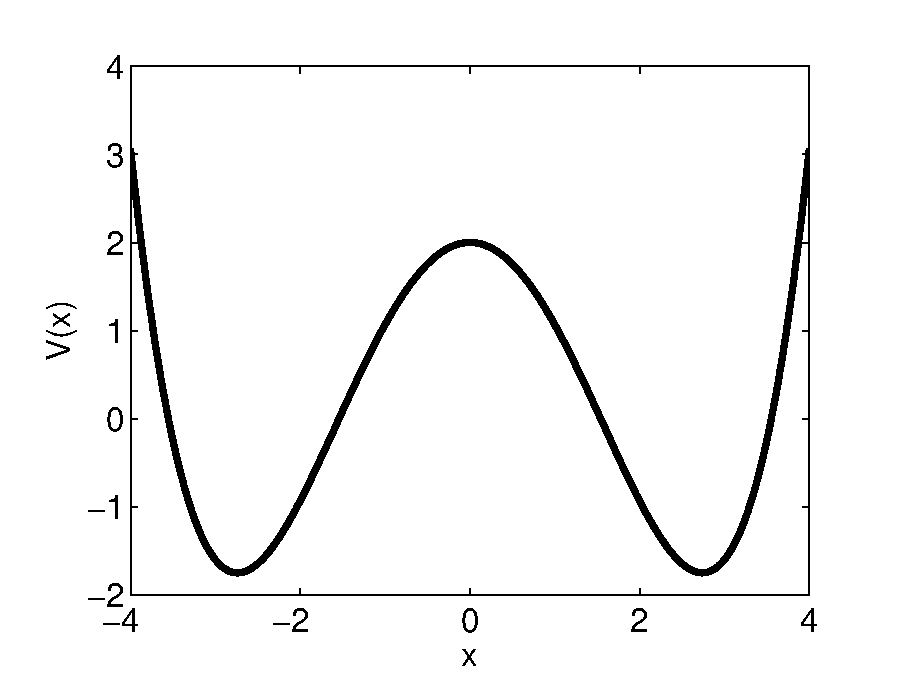
\includegraphics[width=0.5\columnwidth]{potential.eps}
\caption{Her ses et potentiale. Brug denne kommando når I skal
  indsætte figurer. Det er ikke så vigtigt hvor figurer er placeret,
  så længe det er i nærheden af der, hvor I henviser til figuren.}
\label{fig:pot}
\end{center}
\end{figure}

\chapter{Eksempel på Udregninger}
Den kvantemekaniske harmoniske oscillator er en kvantemekanisk
partikel fanget i et potential givet ved
\begin{align}
V(x) = \frac{1}{2} m \omega^2 x^2
\end{align}
Hvis I vil plotte sådan et potential, så se eksemplet i
figur~\ref{fig:pot} (det er et andet potential, som vises i denne
figur). Udregningerne herunder følger \cite{griff}.

Som ved ethvert andet potential starter vi med at finde de stationære tilstande. Vi skal altså løse ligningen
\begin{align}
-\frac{\hbar^2}{2m} \frac{d^2 \psi}{dx^2} + \frac{1}{2}m\omega^2x^2\psi = E\psi
\end{align}
Dette kan løses på 2 måder, hvor løsningerne (selvfølgelig) er
ækvivalente, men alligevel forskellige.

\section{Den analytiske metode}
I denne del af løsningen gælder det om at "brute force" sig til en
(grim) løsning. Dette gøres ved at indføre den dimensionsløse variabel
\begin{align}
\xi = \sqrt{\frac{m\omega}{\hbar}} x
\end{align}
og så omskrive den stationære Schrödingerligning til
\begin{align}
\frac{d^2 \psi}{d \xi^2} = (\xi^2 - K)\psi
\end{align}
med $K = \frac{2E}{\hbar\omega}$. Der løses nu ved hjælp af
potensrækker og der kommes frem til følgende egenenergier
\begin{align}
E_n = \left( n + \frac{1}{2} \right) & \text{ for } n = 0,1,2, \dots
\end{align}
mens der findes frem til følgende egentilstande
\begin{align}
\psi_n = \left( \frac{m\omega}{\pi \hbar} \right)^{1/4}
        \frac{1}{\sqrt{2^n n!}} H_n (\xi) e^{-\xi^2/2}
\end{align}
Her er $H_n(\xi)$ hermite polynomier som til enhver tid kan slåes op i
Schaums \cite{schaums} eller udregnes ved hjælp af formler man også
kan slå op. Grundlæggende er det vigtige blot at det er $n$'te grads
polynomier.

\section{Algebraisk metode}
Opgaven er her at prøve at faktorisere Schrödinger ligningen ved først
at omskrive til
\begin{align}
\frac{1}{2m} (p^2 + (m\omega x)^2)\psi = E\psi
\end{align}
og så førsøge at skrive $(p^2 + (m\omega x)^2)$ som et produkt af to
simple udtryk. Det ville givetvis være nemt hvis ikke $p$ og $x$ var
operatorer. Vi undersøger størrelserne
\begin{align}
a_{\pm} = \frac{1}{\sqrt{2\hbar m \omega}} (\mp i p + m\omega x)
\end{align}
Ved en hurtig udregning ses det at
\begin{align}
a_- a_+ &= \frac{1}{2m\hbar \omega} (p^2 + (m\omega x)^2)\psi 
  - \frac{i}{2\hbar}[x,p] \\
&= \frac{1}{\hbar \omega} H - \frac{i}{2\hbar}[x,p]
\end{align}
hvor $[x,p] = xp - px$ er kommutatoren af $x$ og $p$. En udregning
viser at følgende to udtryk
\begin{align}
[x,p] &= i\hbar \\
[a_- , a_+] &= 1
\end{align}
så derfor får vi nu ligningenerne
\begin{align}
H &= \hbar \omega \left(a_- a_+ - \frac{1}{2} \right) \\
 &= \hbar \omega \left(a_+ a_- + \frac{1}{2} \right)
\end{align}
Ved hjælp af det vises at $a_+$ og $a_-$ kan bruges som stepoperatorer
således at
\begin{align}
H(a_+ \psi) = (E + \hbar \omega) (a_+ \psi) \\
H(a_- \psi) = (E - \hbar \omega) (a_- \psi)
\end{align}
Man vil ikke have negative energier, dvs. det er begrænset hvor mange
gange man kan trække $\hbar \omega$ fra $E$. Det giver, at der findes
en grundtilstand $\psi_0$ så $a_- \psi_0 = 0$ og det kan bruges til at
udregne $\psi_0$. Dermed får man
\begin{align}
\psi_0(x) = \left( \frac{m \omega}{\pi \hbar} \right)^{(1/4)} 
  e^{- \frac{m \omega}{2 \hbar} x^2}
\end{align}
med
\begin{align}
E_0 = \frac{1}{2} \hbar \omega
\end{align}
Man kan nu bruge stepoperatorerne til at udregne de andre egentilstande ved
\begin{align}
a_+ \psi_n = \sqrt{n+1}\psi_{n+1} & & a_- \psi_n = \sqrt{n} \psi_{n-1}
\end{align}
Dermed finder man egentilstandene og egenenergierne
\begin{align}
\psi_n = \frac{1}{\sqrt{n!}} (a_+)^n \psi_0 & & E_n = \left( \frac{1}{2} + n \right) \hbar \omega
\end{align}

\begin{thebibliography}{99}
\bibitem{studieordning} \href{https://mit.au.dk/EDDI/webservices/DokOrdningService.cfc?method=visGodkendtOrdning&dokOrdningId=10727&sprog=da}{Studieordning for bacheloruddannelsen i fysik
  (2015)}.
\bibitem{griff} Introduction to Quantum Mechanics, Second Edition, David J Griffiths.
\bibitem{schaums} Schaums's Mathematical Handbook of formulas and Tables, Third Edition, Murray R Spiegel et.~al.
\end{thebibliography}

\end{document}


